%%% Econ712: Macroeconomics I
%%% Fall 2020
%%% Danny Edgel
%%%
% Due on Canvas Thursday December 10th, 11:59pm Central Time
%%%

%%%
%							PREAMBLE
%%%

\documentclass{article}

%%% declare packages
\usepackage{amsmath}
\usepackage{amssymb}
\usepackage{array}
\usepackage{bm}
\usepackage{changepage}
\usepackage{centernot}
\usepackage{graphicx}
\usepackage[shortlabels]{enumitem}
\usepackage{fancyhdr}
	\fancyhf{} % sets both header and footer to nothing
	\renewcommand{\headrulewidth}{0pt}
    \rfoot{Edgel, \thepage}
    \pagestyle{fancy}
	
%%% define shortcuts for set notation
\newcommand{\Z}{\mathbb{Z}}
\newcommand{\R}{\mathbb{R}}
\newcommand{\Q}{\mathbb{Q}}
\newcommand{\lmt}{\underset{x\rightarrow\infty}{\text{lim }}}
\newcommand{\neglmt}{\underset{x\rightarrow-\infty}{\text{lim }}}
\newcommand{\zerolmt}{\underset{x\rightarrow 0}{\text{lim }}}
\newcommand{\loge}[1]{\text{log}\left(#1\right)}
\newcommand{\usmax}[1]{\underset{#1}{\text{max }}}
\newcommand{\Mt}{M_{t+1}^t}
\newcommand{\vhat}{\hat{v}}
\newcommand{\olp}{\overline{p}}
\renewcommand{\L}{\mathcal{L}}
\newcommand{\olq}{\overline{q}}
\newcommand{\zinf}{_{t=0}^\infty}
\newcommand{\aneg}{A^{-1}}
\newcommand{\sneg}{s^{-1}}
\newcommand{\olk}{\overline{k}}
\newcommand{\olc}{\overline{c}}
\newcommand{\olr}{\overline{r}}
\newcommand{\olpi}{\overline{\pi}}
\newcommand{\Aneg}{A^{-1}}
\renewcommand{\sneg}{s^{-1}}
\newcommand{\dc}[1]{\Delta c_{#1}}
\newcommand{\N}{\mathcal{N}}

\newcommand{\E}[1]{\mathbb{E}\left[#1\right]} % expected value
\newcommand{\Et}[1]{\mathbb{E}_t\left[#1\right]}

%%% define column vector command (from Michael Nattinger)
\newcount\colveccount
\newcommand*\colvec[1]{
        \global\colveccount#1
        \begin{pmatrix}
        \colvecnext
}
\def\colvecnext#1{
        #1
        \global\advance\colveccount-1
        \ifnum\colveccount>0
                \\
                \expandafter\colvecnext
        \else
                \end{pmatrix}
        \fi
}

%%% define function for drawing matrix augmentation lines
\newcommand\aug{\fboxsep=-\fboxrule\!\!\!\fbox{\strut}\!\!\!}

\makeatletter
\let\amsmath@bigm\bigm

\renewcommand{\bigm}[1]{%
  \ifcsname fenced@\string#1\endcsname
    \expandafter\@firstoftwo
  \else
    \expandafter\@secondoftwo
  \fi
  {\expandafter\amsmath@bigm\csname fenced@\string#1\endcsname}%
  {\amsmath@bigm#1}%
}


%________________________________________________________________%

\begin{document}

\title{	Problem Set \#4 }
\author{ 	Danny Edgel 					\\ 
			Econ 712: Macroeconomics I		\\
			Fall 2020						\\
		}
\maketitle\thispagestyle{empty}

%%%________________________________________________________________%%%

\noindent\textit{Collaborated with Sarah Bass, Emily Case, Michael Nattinger, and Alex Von Hafften}

%%%________________________________________________________________%%%
\subsection*{Question 1}

\begin{enumerate}[(a)]
	\item The Bellman equation for the consumer's problem is:
		\[
			V(a,l) = \usmax{a}\left\{\frac{c^{1-\gamma}}{1-\gamma} + \beta\E{V(a',l')}\right\}\text{ s.t. } c + a' \leq wl + (1+r)a 
		\]
		Since the consumer does not value leisure, the budget constraint will hold with equality, and the Bellman becomes:
		\[
			V(a,l) = \usmax{a}\left\{\frac{(wl + (1+r)a - a')^{1-\gamma}}{1-\gamma} + \beta\int V(a',l')Q(l,dl')\right\}
		\]
		We can find the optimality conditions by taking the first order condition of the maximization problem and using the envelope condition:
		\begin{eqnarray*}
			\left(wl + (1+r)a - a'\right)^{-\gamma}(1+r) + \beta\int V'(a',l')Q(l,dl') = 0	\\
			V'(a',l') = \left(w'l' + (1+r')a' - a''\right)^{-\gamma}(-1)	\\
			\left(wl + (1+r)a - a'\right)^{-\gamma}(1+r) = \beta\E{\left(w'l' + (1+r')a' - a''\right)^{-\gamma}}
		\end{eqnarray*}
		In each period,\footnote{Since no decision made by the firm in each period affects its profits in any other period, the firm simply maximizes current-period profits each period.} the firm optimizes according to its profit-maximization problem:
		\[
			\usmax{\{K_t,N_t\}}K_t^\alpha N_t^{1-\alpha} - r_tK_t - w_tN_t
		\]
		Labor supply is exogenously determined, so the firm takes it as given. Then, wages and interest rates are determined to equate capital supply and demand, ensuring that the profit- and utility-maximizing choice of $K_t$ is chosen in each period:
		\begin{align*}
			\alpha K_t^{\alpha-1}N_t^{1-\alpha} - r_t &= 0			\\
			\Rightarrow r_t &= \alpha(N_t/K_t)^{1-\alpha}			\\
			w_t &= \frac{K_t^\alpha N_t^{1-\alpha} - r_tK_t}{N_t}
		\end{align*}
		In equilibrium, capital supply and demand are equal, and interest rates and wages do not depend on the household's state. This equilibrium either cannot be computed analytically or doing so would be prosectuable under the Geneva Conventions. We proceed computationally (see the attached Matlab code), where the final condition of the household problem becomes:
		{\tiny
		\[
			\left(a^\alpha l^{1-\alpha} - (l/a)^{1-\alpha}a + (1+l^{1-\alpha})a^\alpha - a'\right)^{-\gamma}\left(1+\frac{l}{a}^{1-\alpha}\right) = 
			\beta\E{\left(a'^\alpha l'^{1-\alpha} - (l'/a')^{1-\alpha}a' + (1+l'^{1-\alpha})a'^\alpha - a''\right)^{-\gamma}}
		\]
		}%
		\[
			\left((1+l^{1-\alpha})a^\alpha - a'\right)^{-\gamma}\left(1+\frac{l}{a}^{1-\alpha}\right) = 
			\beta\E{\left((1+l'^{1-\alpha})a'^\alpha - a''\right)^{-\gamma}}
		\]
		Since capital markets must clear but the equilibirum capital demand is unknown, we must guess capital demand in equilibrium, use it to calculate wage and interest rates, then retrieve the value function and use its policy function for capital accumulation to determine equilibrium capital supply using the distribution of capital holdings across the unit measure of households. If the two equilibria are not equal, then markets cannot clear and a new guess for capital demand must be used. This results in the following equilibrium:
			\begin{center}
\begin{tabular}{r c}
\hline Capital  & 5.080 \\ 
Interest rate & 0.127 \\ 
Wage & 1.149 \\ \hline
\end{tabular}
\end{center}
	
	\item The probability mass functions of income and consumption are displayed below. You could be forgiven for thinking that these are cumulative distribution functions, given that they appear to be continuously and strictly increasing in consumption and income. This suggests that the overwhelming majority of consumers in this economy are at the higher end of the distribution of consumption and income at any point in time, with a small share of unlucky consumers who drew the low labor state multiple times in a row, eroding their store of assets. 
		\begin{center}
			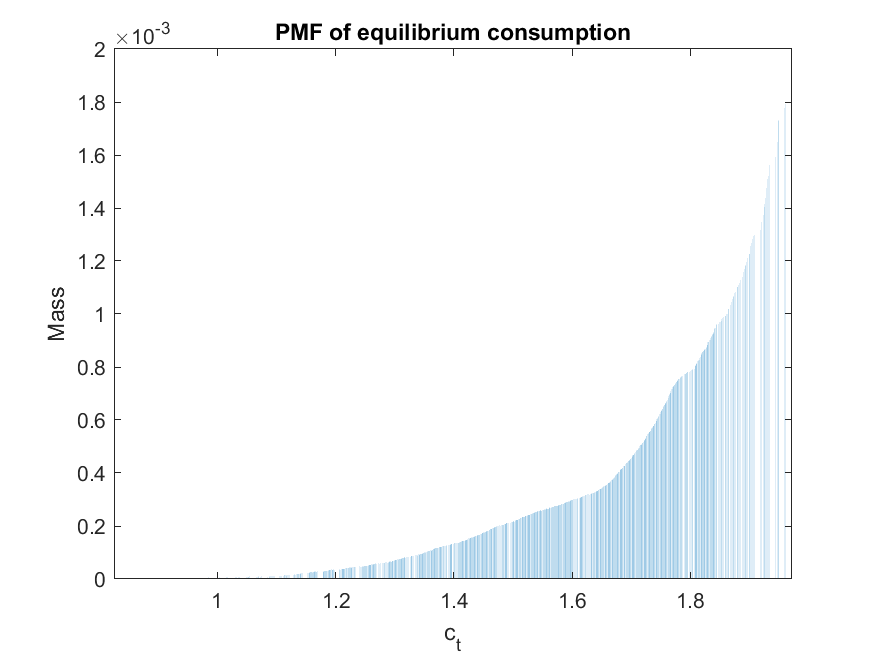
\includegraphics[scale=.35]{figure1bi.png}
			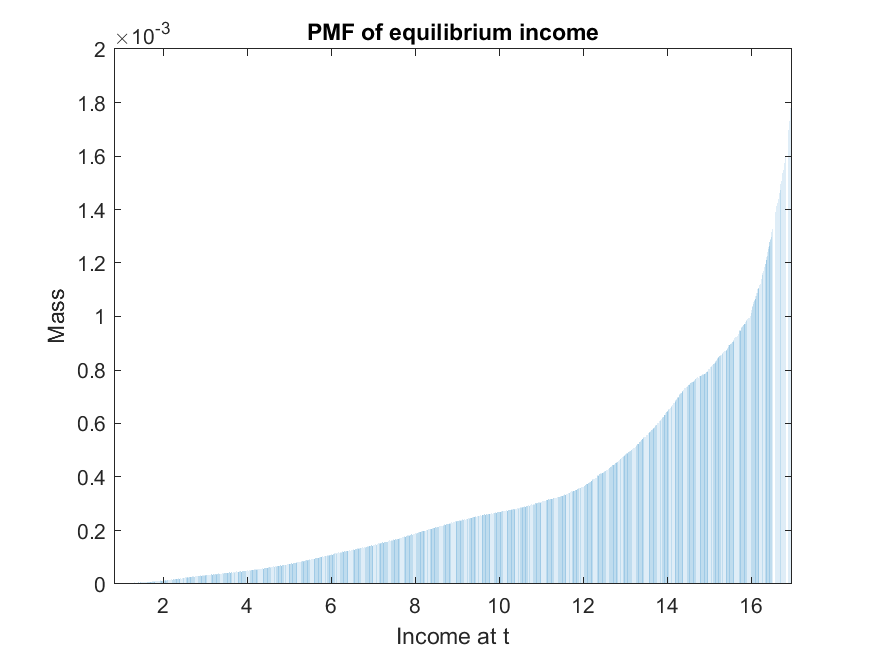
\includegraphics[scale=.35]{figure1bii.png}
		\end{center}
	
	
	\item The equilibrium results with ${a_t\geq-2}$ are displayed in the table below. As you can see, the primary difference between the no-borrowing equilibrium and the borrowing equilibrium is a slight decrease in the capital level, with a slight increase in the interest rate and a slight decrease in the wage rate. This is an intuitive result: Some of the assets held by households with higher holdings will lend their capital to borrowing households rather than to the firm. Thus, the aggregate supply of capital to the firm decreases. Wages relate positively to capital, so they fall relative to the no-borrowing equilibrium, and the firm is willing to pay a higher interest rate when capital supply is lower, so interest rates rise.
		\begin{center}
 \begin{tabular}{r c c}
 & $a_t\geq0$ & $a_t\geq-2$ \\ \hline Capital &  5.080  &  5.010  \\Interest rate &  0.127  &  0.127  \\Wage &  1.149  &  1.143 \\ \hline\end{tabular}
 \end{center}
	
	
\end{enumerate}

%%%________________________________________________________________%%%

\subsection*{Question 2}

\begin{enumerate}[(a)]
	\item The Matlab code provided solves the Bellman equation to find the policy functions for next-period capital and current-period consumption to generate the following plots, comparing them to the deterministic model:
		\begin{center}
			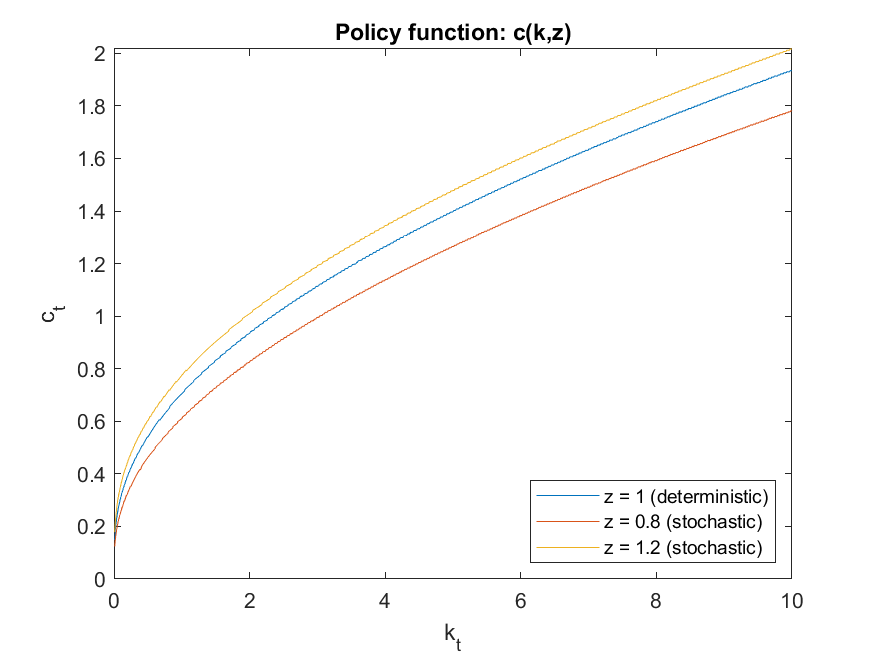
\includegraphics[scale=.35]{figure2ai.png} 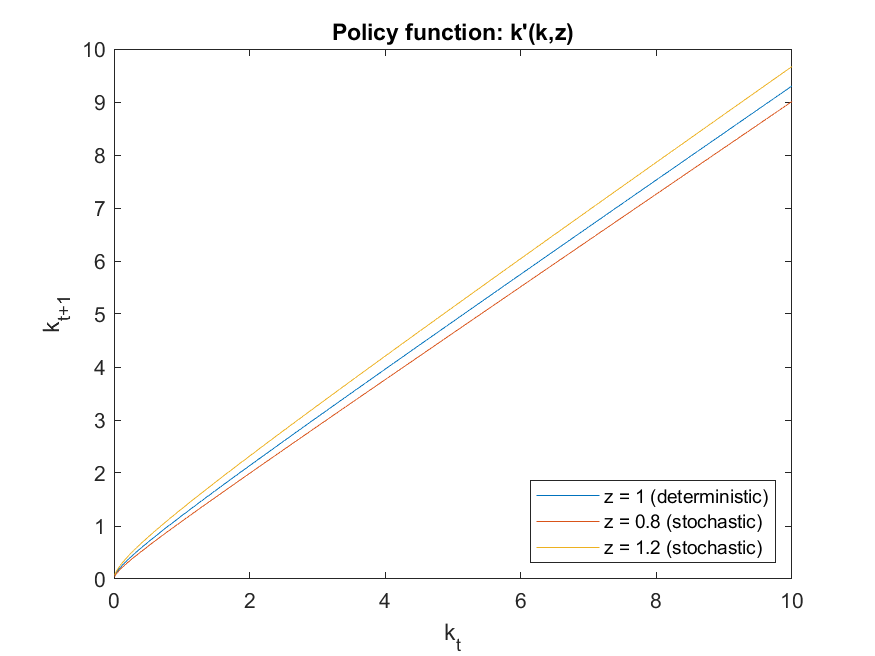
\includegraphics[scale=.35]{figure2aii.png}
		\end{center}
		As you can see, the consumer's optimal policy is to consume more in high-productivity states and less in low-productivity states, with the deterministic optimal consumption between the policy for the two states. The same is true for savings under each scenario.
	
	\item The simulated averages are displayed below, next to the steady-state values from the deterministic model. They generally track, with some noise. In general, investment is higher in the stochastic model, which is consistent with consumers building up greater capital during high-productivity periods in order to smooth consumption between the two periods.
		\begin{center}
\begin{tabular}{r c c}
& Deterministic & Stochastic \\ \hline
Capital  & 3.585 & 3.781  \\ 
Investment & 0.359 & 0.391  \\ 
Consumption & 1.205 & 1.194  \\ 
Interest rate & 0.153 & 0.154 \\ 
Wage & 1.016 & 1.030 \\ \hline
\end{tabular}
\end{center}
	
	
	\item The table below displays the standard deviation of consumption, capital, and output, respectively, along with the correlation betwen consumption and output and the correlation between interest rates and output.
		\begin{center}
\begin{tabular}{r c}
& \\ \hline
$\sigma_c$        & 0.281 \\ 
$\sigma_k$        & 1.423 \\ 
$\sigma_y$        & 0.210 \\ 
$\sigma_{c,y}$    & 0.965 \\ 
$\sigma_{r,y}$    & -0.602 \\ \hline
\end{tabular}
\end{center}
	
	
\end{enumerate}

%%%________________________________________________________________%%%
\pagebreak
\subsection*{Question 3}
The household in this model faces the following optimization problem:
\[
	\usmax{\{c_t\}_{t=0}^\infty}\E{\sum_{t=0}^\infty \beta^tu(c_t)}\text{ s.t }c_t + k_{t+1} - (1-\delta)k_t = (1-\tau)\left(w_tN_t + r_tk_t\right) + T_t + \pi_t
\]
And the firm faces the problem:
\[
	\usmax{\{K_t,N_t\}_t=0^\infty}z_tF(K_t,N_t) - w_tN_t - r_tK_t
\]
And the government faces the following budget constraint:
\[
	T_t \leq \tau(w_tN_t + r_tk_t)
\]

\begin{enumerate}[(a)]
	\item A recursive competitive equilibrium is a continuous, bounded value function, $V(k,K,z)$ for the household; aggregate decision rules, $C(K,z)$, $N(K,z)$, ${K'=G(K,z)}$; and price rules $r(K,z)$ and $w(K,z)$ such that
		\begin{enumerate}[(i)]
			\item $V$ solves the household problem with rules $C$, $N$, and $g$
			\item Price functions $r$ and $w$ are consistent with the firm problem 
			\item Individual and aggregate behavior are consistent: ${g(k,K,z)=G(K,z)}$, ${n(k,K,z)=N(K,z)}$, ${c(k,K,z)=C(K,z)}$
			\item The government budget is balanced: ${T_t = \tau(w_tN_t + r_tk_t)}$
			\item Aggregate feasibility is satisfied: ${C(K,z) + G(K,z) - (1-\delta)K = zF(K,N(K,z))}$
		\end{enumerate}
	
	\item We begin by solving the firm's problem, which does not depend on past or future states and thus is solved in each period with a simple maximization problem with the following first-order conditions:
		\begin{align*}
			r_t &= z_tF_k(K_t,N_t)	\\
			w_t &= z_tF_N(K_t,N_t)
		\end{align*}
		We proceed by defining and solving the Bellman equation for the representative household's problem:
		\[
			V(k,K,z) = \usmax{k'}\left\{u(c) + \beta\E{V(k',K',z')|z}\right\}\text{ s.t. } c + k' = (1-\tau)\left(wN + rk\right) + T + \pi
		\]
		In equilibrium, ${T=\pi=0}$ and ${N=1}$ in all periods. We also know the distribution of $z$. Thus, we can substitute the household budget constraint for household consumption and define its optimization conditions:
		\begin{align*}
			V(k,K,z) &= \usmax{k'}\left\{u((1-\tau)\left(wN + rk\right)-k'+(1-\delta)k+T) + \beta\int V(k',K',z') P(z',z) \right\}
		\end{align*}
		\begin{align*}
			-u'(c) + \beta\int V_k(k',K',z') P(z',z) &= 0					\\
			V_k(k',K',z') &= u'(c')((1-\tau)r'+1-\delta)&\text{(Envelope condition)}	\\
			u'(c) &= \E{\beta u'(c')((1-\tau)r'+1-\delta)|z}
		\end{align*}
		Where the final optimization condition is the Euler equation that must be satisfied by the household's optimal capital accumulation policy.
	
	\item Equilibrium condition (ii) require that ${k=K}$, ${r=zf_K(K)}$, and ${w=zf_N(K)}$, where ${f(K) = F(K,1)}$. These conditions, paired with (iii), (v), and the Euler equation from (b), give us:
		\begin{align*}
			u'(C(K,z)) &= \E{\beta u'(C(K',z'))((1-\tau)zf_K(G(K,z))+1-\delta)|z}	\\
			C(K,z) + G(K,z) - (1-\delta)K &= zf(K)
		\end{align*}
		In each period, all variables in the above equations other than consumption and accumulated capital are given. Thus, we have two equations and two unknowns and the above serves as a functional equation that the aggregate capital accumulation policy must satisty.
	
	\item If ${\delta=1}$, then our aggregate feasibility constraint is ${C(K,z) + G(K,z) = zf(K)}$ and the household's budget constraint in each period\footnote{Assuming zero profits} is ${c + k' = (1-\tau)\left(wN + rk\right) +T}$. Then, our functional equation is:
		\begin{align*}
			u'(C(K,z)) &= \E{\beta u'(C(K',z'))((1-\tau)z'f_K(G(K,z)))|z}	\\
			C(K,z) + G(K,z) &= zf(K)
		\end{align*}
		The social planner's problem in this model is:
		\[
			\usmax{\{c_t\}_{t=0}^\infty}\E{\sum_{t=0}^\infty \beta^tu(c_t)}\text{ s.t } c_t + k_{t+1} = z_tF(K_t,N_t)
		\]
		Where, letting ${N_t=1}$ for all $t$ and substituting the feasibility constraint, the planner's Bellman equation is:
		\[
			V(K,z) = \usmax{k'}\left\{u(zF(k)-k') + \beta\E{V(K',z')|z}\right\}
		\]
		With the following optimization condition (and Euler equation):
		\[
			u'(c) = \E{\beta u'(c')(z'f_k(k')|z}	
		\]
		Thus, when ${\delta=1}$, the social planner's problem and competitive equilibrium have the same feasibility condition, with the following Euler equations:
		\begin{align*}
			u'(c) &= \E{\beta(1-\tau)z'f_k(k')u'(c')|z}	&\text{(CE)}	\\
			u'(c) &= \E{\beta z'f_k(k') u'(c')|z}		&\text{(SPP)}
		\end{align*}
		So the competitive equilibrium's allocation is equal to the social planner's allocation if the social planner optimized using a discount factor that's multiplied by ${1-\tau}$. The interpretation of this result is that a tax, equally applied to all income and redistributed as a lump-sum payment, distorts the competitive equilibrium by lowering the value that agents place on future consumption (i.e. by making them more impatient).
	
\end{enumerate}


%%%________________________________________________________________%%%

\subsection*{Question 4}

\begin{enumerate}[(a)]
	\item Let ${\alpha=\rho}$. Then, the recursive utility function becomes:
		\begin{align*}
			V_t 			&= \left[(1-\beta)c_t^{1-\rho} + \beta\Et{V_{t+1}^{1-\rho}}\right]^{\frac{1}{1-\rho}}	\\
			V_t^{1-\rho} 	&= (1-\beta)c_t^{1-\rho} + \beta\Et{V_{t+1}^{1-\rho}}	
		\end{align*}
		Then, let ${W_t=V_t^{1-\rho}}$ represent risk-adjusted utility:
		\begin{align*}
			W_t	&= (1-\beta)c_t^{1-\rho} + \beta\Et{W_{t+1}} = (1-\beta)c_t^{1-\rho} + \beta\left((1-\beta)c_{t+1}^{1-\rho} + \beta\Et{W_{t+2}}\right)	\\
				&= (1-\beta)c_t^{1-\rho} + \beta(1-\beta)c_{t+1}^{1-\rho} + \beta^2\Et{W_{t+2}}	= ... \\
				&= \sum_{j=0}^\infty \beta^j(1-\beta)c_{t+j}^{1-\rho}
		\end{align*}
	
	\item Notes that, when ${\rho=\alpha}$, we have a utility function with constant intertemporal elasticity of substitution, $\frac{1}{\rho}$. When ${\alpha\neq\rho}$, $\alpha$ only shows up in the exponent of expected future utility. Thus, $\alpha$ is a risk-aversion parameter.
	
	\item $S_t$ is calculated below.
		\begin{align*}
			\frac{\partial V_t}{\partial V_{t+1}} &= \left(\frac{1}{1-\rho}\right)V_t^\rho\left[\beta\left(\frac{1-\rho}{1-\alpha}\right)\left(\Et{V_{t+1}^{1-\alpha}}\right)^{\frac{\alpha-\rho}{1-\alpha}}(1-\alpha)\Et{V_{t+1}^{-\alpha}}\right]	\\
				&= \beta V_t^\rho\left(\Et{V_{t+1}^{1-\alpha}}\right)^{\frac{\alpha-\rho}{1-\alpha}}\Et{V_{t+1}^{-\alpha}} \\
			\frac{\partial V_{t+1}}{\partial c_{t+1}} &= \left(\frac{1}{1-\rho}\right)V_{t+1}^\rho (1-\rho)(1-\beta)c_{t+1}^{-\rho}	\\
				&= \left(1-\beta\right)\left(\frac{V_{t+1}}{c_{t+1}}\right)^\rho	\\
			\frac{\partial V_{t}}{\partial c_{t}} &= \left(1-\beta\right)\left(\frac{V_{t}}{c_{t}}\right)^\rho	\\
\Rightarrow S_t	&= \frac{\beta V_t^\rho\left(\Et{V_{t+1}^{1-\alpha}}\right)^{\frac{\alpha-\rho}{1-\alpha}}\Et{V_{t+1}^{-\alpha}}\left(1-\beta\right)\left(\frac{V_{t+1}}{c_{t+1}}\right)^\rho}{\left(1-\beta\right)\left(\frac{V_{t}}{c_{t}}\right)^\rho}	\\
				&= \beta V_t^\rho \left(\Et{V_{t+1}^{1-\alpha}}\right)^{\frac{\alpha-\rho}{1-\alpha}}\Et{V_{t+1}^{-\alpha}}\left(\frac{V_{t+1}}{V_{t}}\right)^\rho
				\left(\frac{c_{t+1}}{c_{t}}\right)^{-\rho}
		\end{align*}
	
\end{enumerate}
Suppose that consumption growth follows:
\[
	\frac{c_{t+1}}{c_{t}} = g + \sigma_c\varepsilon_{t+1}
\]
Where ${g>0}$, ${\sigma_c>0}$, and ${\varepsilon_t\sim\N(0,1)}$.
\begin{enumerate}[(a)]
	\item Let $s_t$ represent an exogenously-determined shock to the representative agent's endowment at time $t$, dependent on her asset holdings. I conjecture, then, that the price of one asset will depend on $s_t$. Then, we can write the agent's Bellman equation as:
	{\small
		\[
			V(a,s) = \usmax{a'}\left\{\left[(1-\beta)c^{1-\rho}  + \beta\left(\E{V(a',s')^{1-\alpha}}\right)^{\frac{1-\rho}{1-\alpha}}\right]^{\frac{1}{1-\rho}}\right\}\text{ s.t. } c + p(s)a' \leq (p(s) + s)a
		\]
	}%
		At the optimum, the agent's budget constraint will hold with equality. Substituting the constraint for consumption, we can derive the optimality conditions by taking first order conditions:
		\begin{align*}
			-p(s)&(1-\rho)(1-\beta)\left[(p(s) + s)a-p(s)a'\right]^{-\rho} + 	\\
				&\beta\left(\frac{1-\rho}{1-\alpha}\right)\left(\E{V(a',s')}\right)^{\frac{\alpha-\rho}{1-\alpha}}(1-\alpha)\E{V(a',s')^{-\alpha}}V'(a',s') = 0
		\end{align*}
		Where the envelope condition gives us:
		\[
			V'(a',s') = (1-\beta)(p(s')+s')\left[(p(s') + s')a'-p(s')a''\right]^{-\rho}=(1-\beta)(p(s')+s')(c')^{-\rho}
		\]
		Substituting back into the first-order condition and making available cancellations:
		\[
		 p(s)c^{-\rho} = \beta\left(\Et{V(a',s')}\right)^{\frac{\alpha-\rho}{1-\alpha}}\E{V(a',s')^{-\alpha}}(p(s')+s')(c')^{-\rho} 
		\]
		Notice that dividing each side by $c^{-\rho}$ simplify much of the right-hand side of this equation into $S$, the intertemporal marginal rate of substitution that was calculated in 4(c).\footnote{The first 4(c).} Then, the optimality condition becomes:
		\begin{align*}
			p(s) &= \E{\beta S(p(s')+s')}
		\end{align*}
		
	\item A recursive competitive equilibrium is a continuous function, $p(s)$ and a continuous, bounded function, $V(a,s)$, such that:
		\begin{enumerate}[(i)]
			\item $V(a,s)$ solves the Bellman equation 
			\item For all $s$, $V(1,s)$ is attained by ${c=s}$, ${a'=1}$
		\end{enumerate}
	
	
	\item Assume that ${V(c_t) = vc_t}$. Then,
		\begin{align*}
			vc 	&= \usmax{a'}\left\{\left[(1-\beta)c^{1-\rho}  + \beta\left(\E{(vc')^{1-\alpha}}\right)^{\frac{1-\rho}{1-\alpha}}\right]^{\frac{1}{1-\rho}}\right\}	\\
			v	&= c^{\frac{\rho-1}{1-\rho}}\usmax{a'}\left\{\left[(1-\beta)c^{1-\rho}  + \beta\left(\E{\left(v(gc + c\sigma_c\varepsilon')\right)^{1-\alpha}}\right)^{\frac{1-\rho}{1-\alpha}}\right]^{\frac{1}{1-\rho}}\right\}	\\
			v 	&= \usmax{a'}\left\{\left[1-\beta  + c^{(1-\rho)\frac{\alpha-1}{1-\alpha}}\beta\left(\E{\left(v(gc + c\sigma_c\varepsilon')\right)^{1-\alpha}}\right)^{\frac{1-\rho}{1-\alpha}}\right]^{\frac{1}{1-\rho}}\right\}	\\
			v 	&= \usmax{a'}\left\{\left[1-\beta  + \beta\left(\E{\left(v(g+ \sigma_c\varepsilon')\right)^{1-\alpha}}\right)^{\frac{1-\rho}{1-\alpha}}\right]^{\frac{1}{1-\rho}}\right\}
		\end{align*}
		Notice that the value in the maximization statement does not depend on anything controlled by the agent and does not depend on current consumption. Thus,
		\[
			v 	= \left[1-\beta  + \beta\left(\E{\left(v(g+ \sigma_c\varepsilon')\right)^{1-\alpha}}\right)^{\frac{1-\rho}{1-\alpha}}\right]^{\frac{1}{1-\rho}}
		\]
		is a constant.
		
		We can solve for $\loge{S_t}$ simply using the function from 4(c):\footnote{See f.n. 3}
		\begin{align*}
			\loge{S_t} &= \loge{\beta} +  \rho\loge{V_t} + \left(\frac{\alpha-\rho}{1-\alpha}\right)\loge{\Et{V_{t+1}^{1-\alpha}}} + \loge{\Et{V_{t+1}^{-\alpha}}} 	\\
				&+  \rho\loge{\frac{V_{t+1}}{V_{t}}}  - \rho\loge{\frac{c_{t+1}}{c_{t}}}	\\
		\end{align*}
		Letting ${V_t=vc_t}$, we get:
		\begin{align*}
			\loge{S_t} &= \loge{\beta} +  \rho\loge{vc_t} + \left(\frac{\alpha-\rho}{1-\alpha}\right)\loge{\Et{(vc_{t+1})^{1-\alpha}}} + \loge{\Et{(vc_{t+1})^{-\alpha}}} 	\\
				&+  \rho\loge{\frac{c_{t+1}}{c_{t}}}  - \rho\loge{\frac{c_{t+1}}{c_{t}}}	\\
				\loge{S_t} &= \loge{\beta} +  \rho\loge{vc_t} + \left(\frac{\alpha-\rho}{1-\alpha}\right)\loge{\Et{(vc_{t+1})^{1-\alpha}}} + \loge{\Et{(vc_{t+1})^{-\alpha}}}
		\end{align*}
	
	\item The standard CRRA risk-free rate is:
		\[
			R^f_{CRRA} = \frac{1}{\Et{\beta\frac{u'(c_{t+1})}{u'(c_t)}}}
		\]
		Where ${\frac{u'(c_{t+1})}{u'(c_t)}=\left(\frac{c_{t+1}}{c_{t}}\right)^{-\gamma}}$. In our model,we can solve for the risk-free rate by defining our optimal condition as ${1 = \Et{m_tR}}$ and solving for $R$:
		\begin{align*}
			p(s_t) &= \Et{\beta S_t(p(s_{t+1})+s_{t+1})}	\\
			1 &= \Et{\beta S_t\left(\frac{p(s_{t+1})+s_{t+1}}{p(s_t)}\right)} = \Et{\beta S_tR(s_t)}	\\
			R^f(s_t) &= \frac{1}{\Et{\beta S_t}}
		\end{align*}
		This differs from the CRRA case because it depends on the intertemporal MRS rather than on consumption growth, adjusted by the IES.
	
	\item Our pricing kernel for the Lucas tree is ${p(s_t) = \Et{\beta S_t(p(s_{t+1})+s_{t+1})}}$ where, in equilibrium, ${s_t = c_t}$ for all $t$. Then, 
		\begin{align*}
			p(c_t) 	&= \Et{\beta S_t(p(c_{t+1})+c_{t+1})} = \Et{\beta S_t(p(c_t(g + \sigma_c\varepsilon_{t+1}))+c_t(g + \sigma_c\varepsilon_{t+1}))}	\\
					&= \Et{\beta S_tp(c_t(g + \sigma_c\varepsilon_{t+1}))}+ gc_t + c_t\sigma_c\Et{\varepsilon_{t+1}}
		\end{align*}
		Since we know $p(c_t)$ is an expectation function $p(c_t)$ can be separated from the outermost expectation, leaving $\Et{\beta S_t}$, which was shown in (d) to be the reciprocal of the risk-free rate:
		\[
			p(c_t) 	= \frac{p(c_{t+1})}{R^f(s_t)} + gc_t
		\]
		Whereas in the CRRA case, ${p_t = \frac{\Et{x_{t+1}}}{R} + Cov(m_{t+1},x_{t+1})}$. Thus, our case does not substantially differ from the CRRA case; $gc_t$ takes the place of the covariance between next period's divident and the discount factor.
	
	
\end{enumerate}

%%%________________________________________________________________%%%


\end{document}







